\section{Projekt}
Zgodnie z dokumentacją RXHDR\_V1 \cite{master} na szesnastu wyjściach cyfrowych uzyskiwany jest sygnał impulsowy o dodatniej logice cyfrowej z poziomem wysokim wynoszącym +1.8V i czasie trwania między 50ns a 200ns oraz częstotliwości osiągającej nawet do 2.5 MHz.
Sygnał ten na potrzeby dalszej konwersji jest modyfikowany przez translator poziomów do poziomów logicznych 0 - 3.3V i zostaje wybierane osiem kanałów (umownie nazywane: ósemkami) z szesnastu kanałów przez ośmiokanałowy multiplekser.   
Tak wybrane ósemki mają nazwę 1A1-8 dla pierwszej oraz 2A1-8 dla drugiej części wyjść.   
Otrzymane sygnały należy zliczyć za pomocą systemu odczytowego bazującego na płytce Arduino Due w ściśle określonym czasie oraz przekazać dane do dalszej obróbki bądź wizualizacji na zewnętrznym komputerze. 
Schemat wizualizujący powyższy proces transmisji i transformacji sygnału znajduje się na rysunku \ref{projekt chart}.

Proces multipleksowania sygnału z 16 do 8 kanałów wyjść cyfrowych jest konieczny ze względu na wymaganie jakim jest wysoka szybkość zliczania impulsów (2.5MHz/kanał). Wstępne szacowania pokazały że zmniejszenie ilości jednocześnie odczytywanych kanałów będzie konieczne w celu osiągnięcia wymaganej szybkości zliczania. Ten krok dodatkowo znacząco upraszcza projekt płytki dla rozwiązania z wykorzystaniem dodatkowego układu elektronicznego. 
Jednak wersja testowa jaką jest projekt z wykorzystaniem 8 kanałów jest wystarczająca żeby wyznaczyć parametryzację systemu.    

W poniższych rozdziałach opisane są proponowane sposoby rozwiązania zadania binarnych zliczeń w szybkim wielokanałowym układzie. 

\begin{figure}[b]
        \centering
        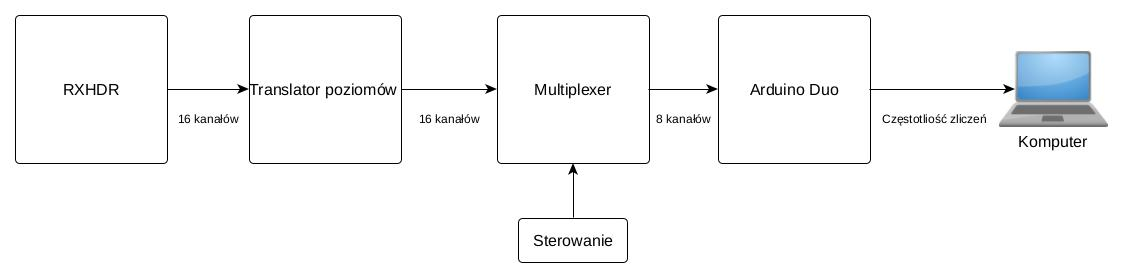
\includegraphics[width=\textwidth]{overwiew_project.jpg}
        \caption{Poglądowy schemat przepływu danych w projekcie licznika binarnego.}
        \label{projekt chart}
\end{figure}

\newpage
\subsection{Rozwiązanie programowe na platformie Arduino}
\label{dzial arduino}
Założeniem rozwiązania jest bezpośrednie zliczenie sygnałów z wykorzystaniem przerwań sprzętowych w frameworku Arduino. W tym celu stosowane są wyjścia cyfrowe płytki Arduino Due oraz multipleksera sygnałów pozwalający na wybranie części z wyjść (1-8,9-16).
Narastające zbocze każdego z tak wybranych sygnałów  powoduje wywołanie krótkiej dedykowanej funkcji zwiększającej zawartość licznika o jeden. 

Fragment kodu \ref{code_ard_IRS} jest częścią programu użytego do badań. Na potrzeby badania zostaje uwzględniony tylko pojedynczy kanał.

\begin{kod}
        \lstinputlisting[language=C++, firstline=95, lastline=117]{code_source/arduino/monocanal_rst.cpp}
        \caption{Fragment kodu użytego do testowania rozwiązania z przerwaniami systemowymi.}
        \label{code_ard_IRS}
\end{kod}

Przebieg akwizycji ukazany jest w powyższym wycinku. Proces ten składa się z następujących kluczowych czynności:
\begin{itemize}
        \item linia 7 - uzyskanie czasu akwizycji z ciągu znaków będących komendą wydawaną przez komputer zarządzający.
        \item linie 8-10 - związanie wystąpienia rosnącego zbocza napięcia na wybranym wejściu z wywołaniem funkcji przerwania \textit{add} (linie 1-3). 
        \item linia 10 - rozpoczęcie procesu zliczania.
        \item linie 13-15 - pętla której zakończenie nastąpi po minięciu czasu akwizycji.
        \item linie 17-20 - powrót do standardowej funkcjonalności mikrokontrolera. Przerwanie zliczania.
        \item linia 21 - wypisanie otrzymanej wartości zliczeń. 
        \item linia 22 - wyzerowanie zawartości zmiennej odpowiedzialnej za przechowywanie wartości zliczeń.     
\end{itemize}

Pomimo krótkiej operacji wewnątrz IRS (ang. \textit{interupt service rutine}) - \textit{add} (kod \ref{code_ard_IRS} linie 1-3, tabela \ref{decompile add}) proces wejścia do procedury przerwania i wyjścia zabiera nieporównywalnie więcej cykli procesora, co powoduje że cały proces wywołania przerwania jest kosztowny w czasie. 
Ilość cykli procesora koniecznych do wywołania funkcji przerwania używając nieoptymalizowanego kodu Arduino może wymagać nawet do 355 cykli procesora \cite{ard_opt_git}, dodatkowo powrót do głównego wątku programu może wymagać kolejnych 128 cykli \cite{ard_opt_git}.

\begin{table}[b]
        \begin{center}
        \caption{Estymacja ilości cykli procesora koniecznych do wykonania instrukcji umieszczonych w funkcji \textit{add} }
        \label{decompile add}
        \begin{tabular}{c|c|c}
                kod C++ & pseudo kod Asemblera & Ilość cykli procesora \cite{cycles} \\ \hline
                val++ & LDR & 1-2 \\
                        & ADD & 1 \\
                        & STR & 1-2 \\ 
                        \hline \hline
                        &   &  3-5 
        \end{tabular}
        \end{center}
\end{table}


Używana płytka rozwojowa Arduino Due, używa mikrokontrolera AT91SAM3X8E w architekturze 32 bitowej o taktowaniu głównego procesora z częstotliwością 84 MHz. Dlatego też pojedynczy cykl procesora zgodnie z wzorem \ref{Cykli w sec} dla układu Arduino Due trwa~$ 11.9 ns $. 
Oznacza to że wykonanie instrukcji \textit{val ++} zgodnie z najgorszą estymacja (tabela \ref{decompile add}) trwa ~ $59.52 ns$. 
Jednak po dodaniu czasu koniecznego na wywołanie i powrót z IRS otrzymywany jest czas $ (355 + 128 + 5) * 11.9 ns =  5.8072 \mu s $. 

Podczas wywołania przerwania o tym samym priorytecie co priorytet tego właśnie wykonywanego, sygnał wywołujący zostanie zapamiętany i ewaluowany zaraz po wyjściu z właśnie wykonywanego IRS  \cite{datasheet}. 
Oznacza to że w przypadku generowania sygnałów o większej częstotliwości niż jest możliwa ich ewaluacja, doprowadzamy do sytuacji kiedy nigdy nie wrócimy do normalnego przebiegu programu. 

Zgodnie z wymaganiami projektu uzyskiwane sygnały wymagające zliczenia mogą przychodzić z częstotliwością nawet do $2.5MHz$ co oznacza kolejny sygnał przychodzący co $0.4\mu s$.
Takie wymagania oznaczają że już dla pojedynczego kanału takie rozwiązanie jest niewystarczające. 

\subsection{Rozwiązanie programowe w standardzie CMSIS}
\label{dzial CMSIS}
Główną filozofią platformy Arduiono jest możliwość przenoszenia kodu między różnymi urządzeniami należącymi do dużej rodziny Arduino oraz łatwość programowania.
W celu osiągnięcia tych dwóch założeń tracona jest optymalizacja w szybkości wykonywalności. 

Dodatkowo platforma Arduino implementuje funkcję których działanie może wpływać na pracę mikrokontrolera nawet bez ich wywoływania. 
Przykładowo na potrzeby działania funkcji \textit{milis()} konieczna jest specyficzna konfiguracja głównego zegara i cykliczne wywoływanie przerwań w celu implementacji licznika. Powoduje to kolejne spowolnienia działania programów. 


CMSIS to biblioteka udostępniająca warstwę abstrakcji dla mikrokontrolerów używających procesorów grupy ARM Cortex. 
Pozwala ona na niskopoziomowe programowanie procesorów tego typu ze skupieniem na szybkości działania.

Zgodnie z notą producenta \cite{interupt latency} w najbardziej optymalnej sytuacji dla procesora \textit{Cortex-M3} wejście do funkcji przerwania sprzętowego wymaga 12 cykli, a wyjście można osiągnąć w 10 cyklach. 
Przy tak optymistycznej estymacji możliwe byłoby osiągnięcie częstotliwości zliczeń nawet do $\frac{1}{11.9ns*27} = ~ 3.11 MHz$, jednak ponieważ zliczenia z różnych kanałów nie mogą być ewaluowane równolegle wynik ten nadal jest niewystarczający. 

Dodatkowo bez dostępu do debugera rozwiązywanie problemów pojawiających się podczas programowania w tym podejściu okazały się niewarte włożonej pracy. 

Z tych dwóch powodów rozwiązanie to zostało porzucone i nie wykonano badań w takim układzie. 

\subsection{Rozwiązanie z użyciem dodatkowego układu elektronicznego przy wykorzystaniu frameworku Arduino.}

W celu osiągnięcia wymaganych założeń projektu zastosowano dodatkowy element elektroniczny mający na celu ułatwienie odczytu zliczeń przez miktrokontroler oraz przeniesienie części z obliczeń na układ elektroniczny.  

\subsubsection{Układ liczników zewnętrznych}
\label{section licziki}

W celu rozwiązania problemu wysokiej częstotliwości zliczeń otrzymywanych z układu RXHDR\_V1 \cite{master} zastosowano zestaw ośmiu binarnych liczników 4-bitowych \cite{licznik doc}. 


\begin{figure}[h]
        \centering
        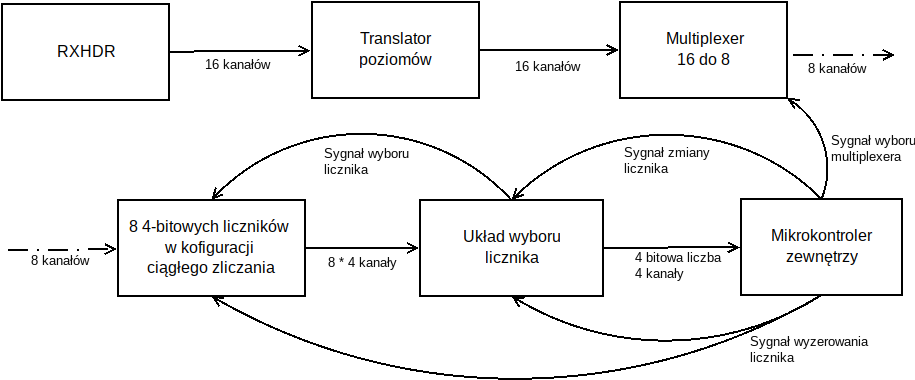
\includegraphics[width=\textwidth]{Elektronika_flow_chart_new.png}
        \caption{Schemat działania układu liczników zewnętrznych i sygnałów kontrolujących}
        \label{licznik flowchart}
\end{figure}

Schemat funkcjonalny układu znajduje się na rysunku \ref{licznik flowchart}.
Na tym diagramie znajdują się sygnały kontrolujące pracę układu. Poniżej zdefiniowane jest nazewnictwo sygnałów na schematach elektronicznych i ich funkcja.  
\begin{itemize}
        \item ReadCLK - Sygnał zmiany licznika - pojedyncze przejście stanu z niskiego na wysoki powoduje wybór kolejnego licznika do odczytu
        \item RC\_B - Sygnał wyzerowania licznika - stan niski powoduje wyzerowanie liczników i ustawienie układów do stanu początkowego.
        \item DIS\_S - Sygnał wyboru multipleksera - Stan logiczny niski powoduje wybranie kanałów 1A1-8 a wysoki 2A1-8
        \item ENP0-7 - Sygnał wyboru licznika - osiem osobnych linii których stan niski pozwala na wybór licznika do odczytu. Podczas odczytu tylko jeden z sygnałów powinien być w stanie niskim reszta powinna utrzymywać stan wysoki. 
        \item DOC\_0-3 - Cztery linie (Czterobitowa liczba) łączące płytkę układu elektronicznego z mikrokontrolerem wyjściowym. Ich stan przekazuje w postaci liczby binarnej zawartość aktualnie wybranego licznika.  
\end{itemize}
Sygnał otrzymywany przez układ RXHDR\_V1 jest przepuszczany przez translator poziomów w celu zmiany logiki z 0-1.8$V$ do 0-3.3$V$. Następnie z 16 kanałów zostaje wybrane 8, tak opracowane sygnały trafiają na układ liczników.

\paragraph{Układ liczników \cite{licznik doc}\cite{slave}}

\begin{figure}[]
        \centering
        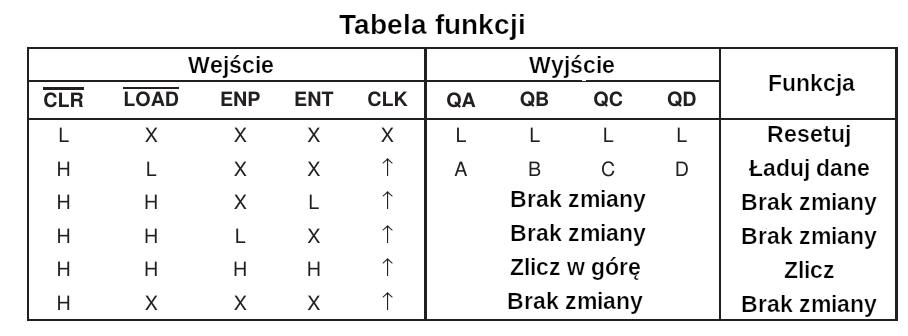
\includegraphics[width=0.8\textwidth]{licznik_tabela_prawdy.png}
        \caption{Tabela funkcji licznika binarnego SN74LV161A \cite{licznik doc}}
        \label{licznik tabela funkcji}
\end{figure}

4-bitowy binarny licznik SN74LV161A ma 9 wejść logicznych. 
W tym układzie licznik znajduje się w następującej konfiguracji:
\begin{itemize}
        \item $CLK$ - Wejście zliczające przychodzące impulsy. Każde narastające zbocze impulsu powoduje zwiększenie wartości przechowywanej w liczniku aż do momentu przepełnienia licznika kiedy to następuje przepełnienie i przechowywana wartość jest zerowana.  
        \item $\overline{CLR}$ - Połączone z linią RC\_B, stan niski powoduje wstrzymanie pracy i wyzerowanie wartości przechowywanych w liczniku. 
        \item $ENT,ENP$ - w celu stabilizacji układu na czas odczytywania wartości chcemy wstrzymać zliczanie, dlatego też ustalamy stan wysoki dla wejścia ENT i wejście ENP łączymy z kanałem ENP0-7 odpowiadającym odpowiedniemu licznikowi.
        
        Podczas wyboru licznika (czyli w chwili odczytu wartości przechowywanych w liczniku) ustalana jest wartość niska na odpowiadającym kanale ENP uzyskując stan zablokowania licznika. 
        Sprawia to że wraz z wyborem licznika układ ustala swój stan i nie zmienia go aż do chwili wyboru następnego. 
        W ten sposób unikane są niepewności i błędy wynikające z odczytywania zmieniającej się wartości. Niestety skutkiem ubocznym takiego podejścia jest powstanie czasu martwego w układzie podczas którego wartości nie będą zliczane na odczytywanym liczniku.
        \item $A,B,C,D$ - Wejścia pozwalające ustawić dowolną wartość startową licznika. W przypadku tej pracy wartość wszystkich czterech bitów jest ustawiona na niski stan logiczny.
        \item $\overline{LOAD}$ - funkcja ładowania wartości, nie jest (używana wejście to jest uziemione).
\end{itemize} 
Tabela prawdy dla powyższych wejść 4-bitowego binarnego licznika SN74LV161A znajduje sie na rysunku \ref{licznik tabela funkcji}

W ustalonej konfiguracji wykorzystane są jedynie linie Q0-3 to one podają binarnie przechowywaną wartość. 
Tak skonfigurowane liczniki będą zliczać wartości otrzymywane przez wejście $CLK$ aż do otrzymania 16-tego impulsu kiedy to licznik zostaje przepełniony i podawana przez niego wartość wraca do 0. 

\paragraph{Układ wyboru sygnału}

Celem tego układu jest przełożenie rosnącego zbocza na linii ReadCLC (sygnał zmiany licznika) na konfigurację zestawu liczników (sygnał wyboru licznika) pozwalającą na odczyt wartości w kolejnym liczniku. W tym celu wykorzystany jest rejestr przesuwany. 
Wybrany układ służący temu zadaniu to SN74LV164A\cite{shift doc}, jest on szeregowo-równoległym rejestrem co oznacza że dane wejściowe są dostarczane szeregowo a otrzymywana jest informacja równoległa która jest przesuwana wraz z kolejnymi sygnałami zegara. Dokumentacja rejestru SN74LV164A mówi o dwóch wejściach jednak są one bezpośrednio wyprowadzane na bramkę logiczną AND co sprawia że układ ten spełnia warunek pojedynczego wejścia rejestru szeregowo-równoległego. W konfiguracji tego układu gdzie oba wejścia są ze sobą zwarte, bramka logiczna AND jest ignorowana.
Schemat układu wyboru licznika znajduje się rysunku \ref{wybor schema}. 

\begin{figure}
        \begin{multicols}{2}
                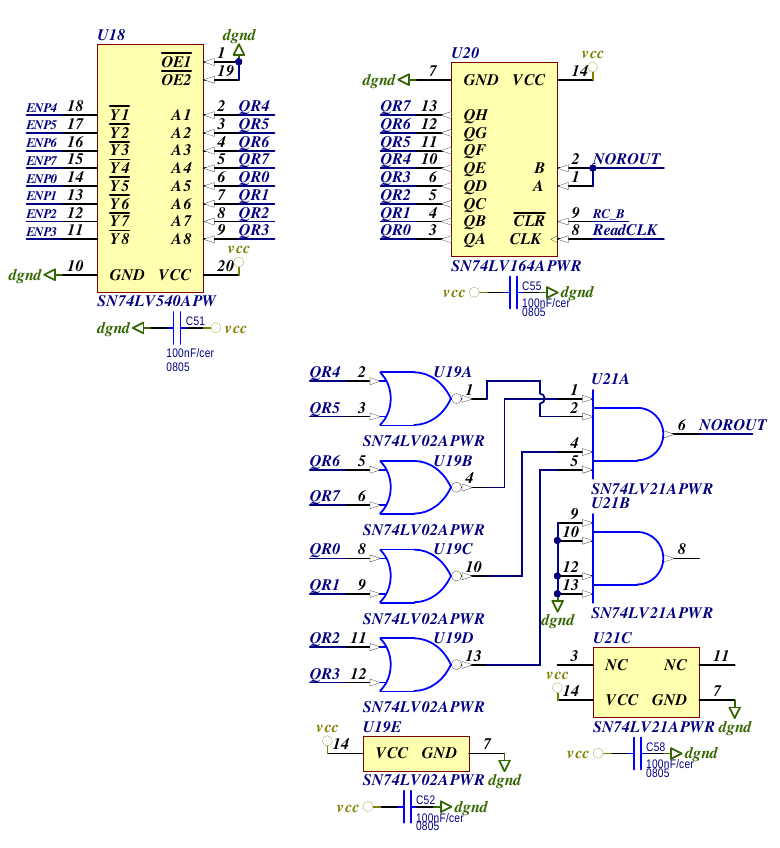
\includegraphics[width=0.45\textwidth]{shift_register.png}
                \caption{Schemat układu wyboru licznika wykorzystujący rejestr przesuwny.}
                \label{wybor schema}
                \par
                \hfill
                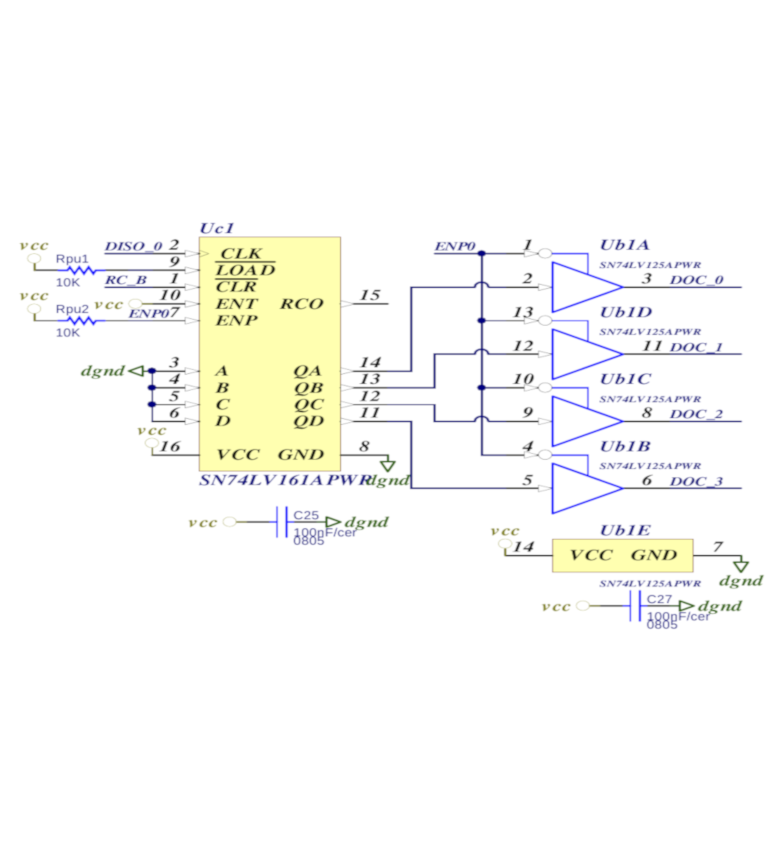
\includegraphics[width=0.45\textwidth]{Licznik.png}
                \caption{Schemat konfiguracji jednego z używanych liczników wraz z częścią multipleksera wyjściowego.}
                \label{licznik}
                \par
                \hfill
        \end{multicols} 
\end{figure}

W celu osiągnięcia efektu pojedynczej wartości logicznej która przesuwa się z każdym rosnącym zboczem sygnału na wejściu rejestru musimy dostarczyć pojedynczy wysoki stan podczas pierwszego cyklu pracy, a następnie trzymać stan niski aż do chwili potrzeby powtórzenia cyklu. 
Za pomocą bramek NOR układu SN74LV02A oraz bramek AND układu SN74LV21A ustalonych zgodnie ze schematem na rysunku \ref{wybor schema} osiągamy równanie logiczne:
\begin{equation}
        NOROUT = \overline{(QR1+QR2)} * \overline{(QR3+QR4)} * \overline{(QR5+QR6)} + \overline{(QR7+QR8)}
\end{equation}
Gdzie:
\begin{itemize}
        \item $NOROUT$ - Sygnał wejściowy rejestru 
        \item $QR1-8$ - Wyjścia rejestru. 
\end{itemize}

\begin{table}
        \centering
        \caption{Cykl działania rejestru przesuwnego układu wyboru licznika}
        \label{shift sygnal}
        \begin{tabular}{lccccccccc}
                Czas &$QR1$&$QR2$&$QR3$&$QR4$&$QR5$&$QR6$&$QR7$&$QR8$  &NOROUT\\ \hline     
                T1&L&L&L&L&L&L&L&L &H\\
                T2&H&L&L&L&L&L&L&L &L\\
                T3&L&H&L&L&L&L&L&L &L\\
                T4&L&L&H&L&L&L&L&L &L\\
                T5&L&L&L&H&L&L&L&L &L\\
                T6&L&L&L&L&H&L&L&L &L\\
                T7&L&L&L&L&L&H&L&L &L\\
                T8&L&L&L&L&L&L&H&L &L\\
                T9&L&L&L&L&L&L&L&H &L\\
                T10&L&L&L&L&L&L&L&L &H\\
        \end{tabular}
\end{table}

Sekwencja sygnału pokazana jest w tabeli \ref{shift sygnal}. Na tej wizualizacji widać że gdyby w konfiguracji zastąpić linię $QR8$ połączeniem do stanu logicznego niskiego (uziemienia) możliwe byłoby ograniczenie liczby sekwencji w cyklu do 8. Jednak dzięki tej pojedynczej sekwencji gdy żaden z liczników nie jest odczytywany otrzymujemy cykl podczas którego żaden z liczników nie jest zablokowany i wszystkie kontynuują liczenie. 

W ten sposób otrzymywany sygnał następnie jest negowany przez układ SN74LV540 i dostarczany do multipleksera pokazanego na rysunku \ref{licznik}.

Zgodnie z tabelą funkcji \ref{licznik tabela funkcji} oraz schematem na rysunku \ref{licznik} można stwierdzić że stan niski ENP0-7 powoduje konfigurację licznika powodująca wstrzymanie zliczania oraz wyprowadzenie wyjścia tego licznika na linie odczytu mikrokontrolera. Przeciwny stan (wysoki) lini ENP0-7 powoduje przywrócenie funkcji zmiany wartości przechowywanej w liczniku i oddziela stan licznika od lini wyjściowych. 

Funkcję odcięcia stanu licznika od lini DOC\_0-3 uzyskiwany jest poprzez użycie cyfrowych bramek buforujących umieszczonych w układzie  SN74LV125APWR \cite{buffer}.
 

\paragraph{Czas martwy i szybkość odczytu układu licznika}

Podczas odczytu licznika informacja o zliczeniach zostaje tracona oznacza to że układ ten generuje czas martwy. 
Procentowa długość tego czasu może być wyznaczona na podstawie wzoru:
\begin{equation}
        T_d = \frac{T_o/N_l}{T_o+T_e} * 100\%
\end{equation}
Gdzie:
\begin{description}
        \item $T_d$ - procentowy czas martwy licznika.
        \item $T_o$ - czas odczytu.
        \item $N_l$ - liczba liczników w sekwencji odczytu. W używanej konfiguracji jest to osiem liczników. 
        \item $T_e$ - czas pustego cyklu.
\end{description}

Oznacza to że przedłużając czas pustego cyklu zmniejszamy czas martwy układu, jednak ponieważ liczniki mogą jedynie 16 stanów to konieczne jest odczytanie ich przed zliczeniem 16 liczby. 
Oznacza to że:
\begin{equation}
        T_o+T_e * F \leqslant 15
\end{equation}
        Gdzie:
\begin{description}
        \item $F$ - spodziewana częstotliwość zliczeń
\end{description}

Dla podanych wymagań: 2.5 miliona zliczeń na sekundę, można wyliczyć że suma czasu odczytu i pustych sekwencji powinna być mniejsza niż 6$\mu s$.
Oznacza to że sekwencja odczytu powinna zmieścić się w 504 cyklach procesora. 

\subsubsection{Oprogramowanie mikrokontrolera}
\label{oprogramowanie mikrokontrolera}

Zadaniem mikrokontrolera jest odebranie danych z układu wspomagającego w czasie uniemożliwiającym przepełnienie liczników i wysłanie sformatowanych danych na komputer zewnętrzy. 

Cały proces kompilacji kodu C++ do kodu Asemblera został wykonany na kompilatorze ARM gcc 4.6.4 (linux). 

\paragraph{Wymagane połączenie}
W celu utworzenia funkcjonującego układu akwizycji zliczeń konieczne jest połączenie kablem USB2.0 typ A/micro-USB typ B między komputerem sterującym a natywnym portem Arduino Due (Port bliżej przycisku resetu).

Dodatkowo wymagane jest połączenie z płytką zewnętrzną. Konieczne połączenia to:
\begin{itemize}
        \item Połączenia $DOC\_0-3\_ext$ w domyślnej konfiguracji powinny być połączone z wyjściami arduino o pinach 33-36 - są to wyjścia liczników.
        \item $ReadCLC$ - arduino pin 25 - wyjście sygnału zmiany licznika
        \item $RC\_B\_ext$ - arduino pin 26 - wyjście sygnału resetu liczników 
        \item $DIS\_S\_ext$ - arduino pin 27 - wyjście sygnału wyboru multipleksera
        \item $LOW\_RATE\_ext$ - arduino pin 28 - wyjście sygnału dla części analogowej układu wyboru LOW\_RATE
        \item $ENBLR\_ext$ - arduino pin 30 - wyjście sygnału dla części analogowej układu wyboru ENBLR 
        \item Dodatkowo koniecznie jest ustalenie wspólnego uziemienia w celu stabilizacji poziomów logicznych.
\end{itemize}

Są to wyjścia w domyślnej konfiguracji i można dokonać zmiany poprzez modyfikację pliku \textit{USER\_CONFIG.h}.



\paragraph{Akwizycja danych}
Dane otrzymywane z zewnętrznego układu elektronicznego (dział \ref{section licziki}) mają postać binarnej liczby 4-pozycyjnej rosnącej do wartości 15 a następnie zawijające się ponownie do liczby 0. 
Dzięki tej formie prezentacji danych po odczytaniu stanów logicznych na urządzeniu peryferyjnym i odpowiednim przesunięciu logicznym w prosty sposób otrzymujemy wartość na liczniku. 
Podejście to jednak wymaga specyficznego połączenia oraz uwzględnienia potencjalnego przepełnienia licznika. 

W jednym cyklu akwizycji zostaje wybierany pierwsze osiem kanałów 1A1-8 następnie przez czas akwizycji, korygowanej o czas martwy, zbierane są dane z liczników i dodawane do miejsca w tablicy odpowiadającemu odpowiedniemu licznikowi, następnie zmieniana jest ósemka badanych kanałów i proces ponownie jest powtarzany. 

Proces akwizycji danych musi być bardzo dokładnie kontrolowany pod względem czasu wykonania.
Czas pobierania danych jest regulowany przez ilość pętli podczas których dokonywana jest akwizycja danych. 
Przykład tej pętli znajduje się w fragmencie kodu \ref{code aqw}.

\begin{kod}
        \lstinputlisting[language=C++, firstline=85, lastline=115]{code_source/arduino/final.cpp}
        \caption{Fragment kodu odpowiedzialnego za akwizycję danych}
        \label{code aqw}
\end{kod}

Jak widać ilość iteracji jest ustalana przez wymagany czas w milisekundach po korekcjach o czas martwy licznika oraz z uwzględnieniem ilości czasu przypadającego na pojedynczą pętlę (kod \ref{code aqw} linia 1). 
Warunkiem koniecznym takiego podejścia jest stały czas wykonywania iteracji pętli. 
Różnice w czasie mogą być powodowane przez operacje dostępu do pamięci kiedy to w różnych iteracjach stosujemy dostęp do pamięci a w innych wykorzystujemy wcześniej przygotowane rejestry.
Drugim powodem mogą być rozwidlenia pracy programu, sytuacje kiedy przebieg programu jest uwarunkowany wynikiem jakiegoś warunku i dwie drogi potrzebują różną ilość cykli procesora na wykonanie. 
W celu analizy takich sytuacji przydatna jest analiza skompilowanego kodu c do kodu asemblera.
Fragment krytycznej części programu (kod \ref{code aqw} linie 3-25) jest przedstawiony w wycinku kodu \ref{asembly}.

\begin{kod}
        \lstinputlisting[language={[Motorola68k]Assembler},firstline=30, lastline=48]{code_source/asembler/loop_final.S}
        \caption{Fragment kodu asemblera utworzonego przez kompilację części kodu \ref{code aqw}. }
        \label{asembly}
\end{kod}

Po analizie kodu \ref{asembly} można stwierdzić że nie zdarza się sytuacja żeby w różnych iteracjach występowała różna ilość dostępów do pamięci.
Jak widać w fragmencie programu \ref{code aqw} linie 16-21 w przypadku wystąpienia przepełnienia licznika konieczne jest dodanie wartości pełnego licznika do otrzymanej liczby. 
Powoduje to że wymagana jest dodatkowa instrukcja add.

Jednak proces warunkowego dodania jest realizowany przez specyficzną instrukcję it (kod \ref{asembly} linie 10-14).
Należy ona do zestawu instrukcji Thumb®-2 i pozwala na uniknięcie problemów wynikających z warunkowej zmiany biegu programu dla krótkich instrukcji. 
Zgodnie z dokumentacją\cite{cycles} cortex-M3 czas potrzebny na wykonanie tej instrukcji to jeden cykl procesora, jednak jest sprecyzowane że instrukcja może być dołączona do następnej instrukcji pozwalając na wykonanie w tym samym czasie co następna komenda.
Tak się dzieje w przypadku spełnienia warunku gt (ang. \textit{greater then} - większy niż) poprzedniej instrukcji cmp (linie 9-10). Jednak jeżeli warunek ten nie zostaje spełniony to ewaluacja instrukcji it zwiększa się do jednego cyklu i przechodzi do warunku else (druga instrukcja w kolejności).
Cały ten proces sprawia że tak samo w przypadku spełniania warunku gt jak i w przypadku niezgodności ten fragment kodu wymaga dwóch cykli procesora.
$$it(1c) + rsb(1c) = it(0c) + add(1c) + rsb(1c)$$

Dodatkowym wymogiem jest stały czas wykonywania pętli dla wszystkich kanałów. Gdyby któryś z kanałów różnił się czasem przebiegu również różniłby się czasem martwym dla konkretnego kanału. Powodowałoby to różną wydajność. 
Analiza na oscyloskopie dowiodła że czas blokowania licznika dla ostatnich kanałów (8,16) jest krótszy niż czas dla pozostałych przypadków. Dlatego też w celu korekcji tej różnicy po zakończeniu pętli (kod \ref{code aqw} linia 27) przed wkroczeniem do pustego cyklu umieszczone zostały puste instrukcje NOP które regulują długość czasu martwego dla tych kanałów. 


\paragraph{Komunikacja z komputerem zewnętrznym}
Ze względu na fakt że proces akwizycji danych jest tak wrażliwy na wszelkie zmiany ilości poleceń konieczne jest wyłączenie obsługi przerwań w trakcie wykonywania kluczowego fragment programu. 
Sprawia to że w trakcie akwizycji obsługa komunikacji z zewnętrznymi urządzeniami przez układy komunikacji seryjnej jest niemożliwa. 
Oznacza to że wymagana jest bardzo dokładna obsługa komunikacji z zwróceniem szczególnej uwagi na potencjalne błędy. 

W tabeli \ref{komunikacja} znajdują się komendy i odpowiedzi stosowane w komunikacji między urządzeniami. 
Forma wszelkich stałych komunikacyjnych znajduje się w osobnym pliku \textit{USER\_CONFIG.h} pozwalającym na łatwą zmianę prezentowanych komend.

W tabeli \ref{komunikacja} przedstawione są dodatkowe komendy pozwalające na kontrolę funkcjonalności i konfiguracji układu RXHDR\_V1. Są to sygnały LOW\_RATE oraz ENBLR funkcjonalnością tych sygnałów zawarta jest w dokumentacji RXHDR\_V1 \cite{master}.

\begin{table}
        \centering
        \caption{Tabela komend stosowanych w celu komunikacji między komputerem zewnętrznym a mikrokontrolerem}
        \label{komunikacja}
        \begin{tabularx}{\textwidth}{|c|c|X|}
                \hline
                komenda & odpowiedź & opis \\ \hline

                \textbackslash n & Ready to read\textbackslash n & 
                Krótki znak rozpoczynający komunikację.
                Po otrzymaniu tego symbolu mikrokontroler wstrzymuje proces akwizycji i oczekuje na dalsze polecenia.
                Przed wysłaniem dowolnej komendy konieczne jest poprzedzenie tym symbolem, w celu upewnienia się że mikrokontroler jest gotowy na zmianę trybu pracy.
                \\ \hline

                42a\textbackslash n & 42b\textbackslash n& Krótka komenda, nie zmieniająca nic w pracy licznika. Pozwala na sprawdzenie komunikacji między licznikiem a komputerem zewnętrznym. \\ \hline

                atm\textbackslash TIME\textbackslash n & TIME\textbackslash n& TIME to czas w milisekundach, jest on ustalany jako czas akwizycji licznika. Musi on być podany jako liczba całkowita.\\ \hline

                stp\textbackslash n& fin\textbackslash n& Wstrzymuje pracę licznika. \\ \hline

                srt\textbackslash n& - & Rozpoczyna pracę licznika \\ \hline

                ltr\textbackslash nVAL\textbackslash n& VAL\textbackslash n & Ustawienie poziomu logicznego odpowiadającego wartości VAL (1 - wysoki poziom, 0 - niski poziom) na wyjściu odpowiadającemu ustawieniu LOW\_RATE analogowej części licznika. \\ \hline
                
                enr\textbackslash nVAL\textbackslash n& VAL\textbackslash n & Ustawienie poziomu logicznego odpowiadającego wartości VAL (1 - wysoki poziom, 0 - niski poziom) na wyjściu odpowiadającemu ustawieniu ENBLR analogowej części licznika. \\ \hline

        \end{tabularx}
\end{table}

Po zakończonej akwizycji dane zostają wysłane w jednym kawałku na komputer zewnętrzny w postaci:
\begin{itemize}
        \item \detokenize{<~+~>}'\textbackslash n'
        \item {Nazwa kanału}'\textbackslash t'{wynik}'\textbackslash n'
        \item \detokenize{~<+>~}'\textbackslash n'
\end{itemize}
Przykład komunikacji wygląda następująco:
\begin{lstlisting}
<~+~>
1A1     1234
1A2     1234 
    ...
2A8     1234
~<+>~
\end{lstlisting}

Długi symbol początku i końca danych pozwala na łatwe odnalezienie fragmentu komunikacji które zawiera dane pomiarowe. Dodatkowo długość symboli sprawia że wszelkie komplikacje w komunikacji będą wykrywanie co zmniejsza szansę na akwizycję błędnych danych. 

\subsection{Program kontroli, wizualizacji oraz archiwizacji danych}

Program używany na komputerze podłączonym do mikrokontrolera został napisany z wykorzystaniem języka Python i frameworku PyQt5.
Szczegółowe zadania programu to:
\begin{itemize}
        \item Komunikacja z mikrokontrolerem w celu:
        \begin{itemize}
                \item upewnienia się o sprawnym działaniu programu na płytce arduino,
                \item ustawienia czasu akwizycji,
                \item odebraniu danych o zliczeniach. 
        \end{itemize}
        \item Umożliwienie wyboru konfiguracji pracy programów przez interfejs użytkownika.
        \item Analiza otrzymanych danych pomiarowych.
        \item Wizualizacja danych pomiarowych.
        \item Archiwizacja danych pomiarowych w wybranym formacie danych.
\end{itemize}

Program podzielony jest na dwie zależne od siebie części. Fasadę (ang. front-end) zawierającą graficzny interfejs użytkownika (ang. GUI) oraz wnętrze (ang. back-end).

\paragraph{Wnętrze}

Głównym celem tej części programu jest komunikacja z mikrokontrolerem. 
W tym celu wykorzystywana jest biblioteka PySerial\cite{pyserial} pozwalająca na łatwą obsługę portu szeregowego USB. 

By umożliwić jednoczesną wizualizację danych wraz z odbieraniem informacji z mikrokontrolera konieczna była implementacja wątku zajmującego się ciągłym odbiorem danych. 
Dlatego też jedyny cel funkcji \textit{back\_end\_deamon} jest nasłuchiwanie w ciągłej pętli oraz zapisywanie danych w logu komunikacyjnym (\textit{RawLogClass}). 
Na podstawie klasy tego logu wątek główny programu okresowo aktualizuje klasę \textit{CountRateData} która jest wykorzystywana przez fasadę (\textit{gui\_module}) w celu wizualizacji. 

Klasa \textit{CountRateData} oprócz przetrzymywania danych o zliczeniach dla każdego kanału również zawiera informacje o czasie akwizycji, dzięki temu możliwe jest przekazywanie informacji do wizualizacji już jako częstotliwości zliczeń. 

Dodatkową funkcjonalnością programu jest możliwość przeprowadzenia pojedynczego badania nazywanego \textit{Single Shoot} lub skrótowo \textit{ss}.
Funkcja ta pozwala na wizualizację w postaci wykresu słupkowego pojedynczego badania w przeciwieństwie do domyślnego układu wizualizacji który jest stale aktualizowany. 
W celu przeprowadzenia takiego pomiaru wątek \textit{get\_ss\_mesurements} zamyka mutexy odpowiedzialne zasoby sprzętowe jakim jest za port seryjny oraz zasób danych znajdujący się w zmiennych klasy logu. 
Tym sposobem wstrzymywane są inne funkcje programu aż do zakończenia pomiaru \textit{Single Shoot}.
Pomiar kończy się komendą wstrzymania pracy licznika pozwalając na zmianę konfiguracji przed kolejnymi pomiarami. Informacje konfiguracyjne znajdują się w instancji klasy \textit{ConfigurationData}. Zadaniem fasady jest zmiana wartości pól tej klasy w chwili gdy użytkownik wprowadzi nowe parametry pomiarów. 

Schemat elementów programu wraz z mutexami które chronią przed błędami jednoczesnego dostępu zwizualizowane są na rysunku \ref{program zapotrzebowanie}.
\begin{figure}
        \centering
        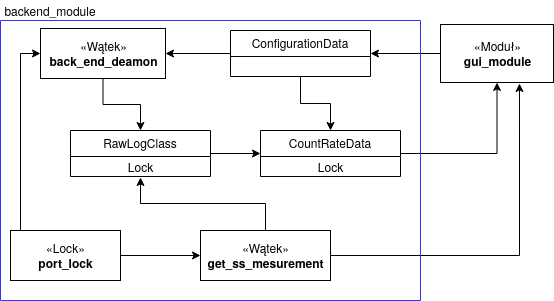
\includegraphics[width=0.65\textwidth]{Schemat_zapotrzebowania.png}
        \caption{Schemat zapotrzebowania na zasoby przez elementy programu}
        \label{program zapotrzebowanie}
\end{figure}


Dane pomiarowe są zapisywane w chwili gdy: Program zostanie zamknięty, wciśnięty zostanie guzik \textit{force save}, lub minie czas auto zapisu ustawiany w interfejsie użytkownika. 

Przed zapisem tworzony zostaje folder z aktualną datą, w formacie DD-MM-YYYY, w wybranej przez użytkownika ścieżce. Nazwa pliku to godzina zapisu pliku w formacie HH:MM:SS
Pliki są zapisywane w ustalonym formacie: JSON lub CSV.

Archiwizacja danych z akwizycji \textit{Single Shoot} jest przeprowadzana zaraz po zakończeniu pomiaru w osobnym folderze zgodnie z wcześniej przedstawioną zasadą. 

\paragraph{Fasada}
\begin{figure}
        \begin{multicols}{2}
        
        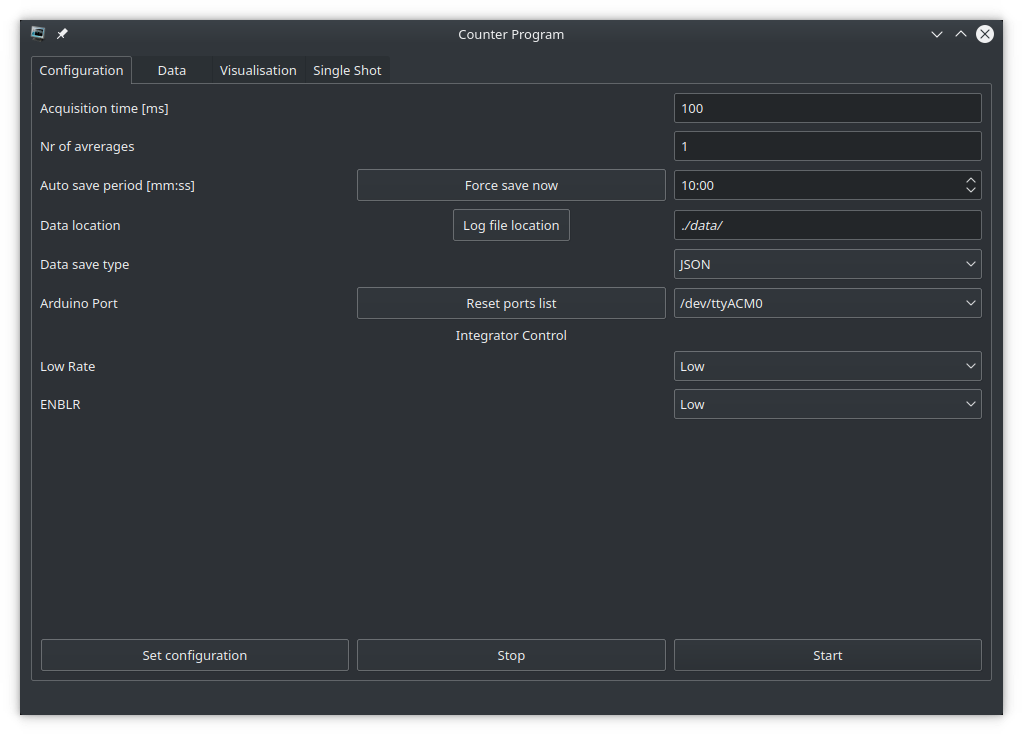
\includegraphics[width=0.49\textwidth]{GUI_config.png}\par
        
        
        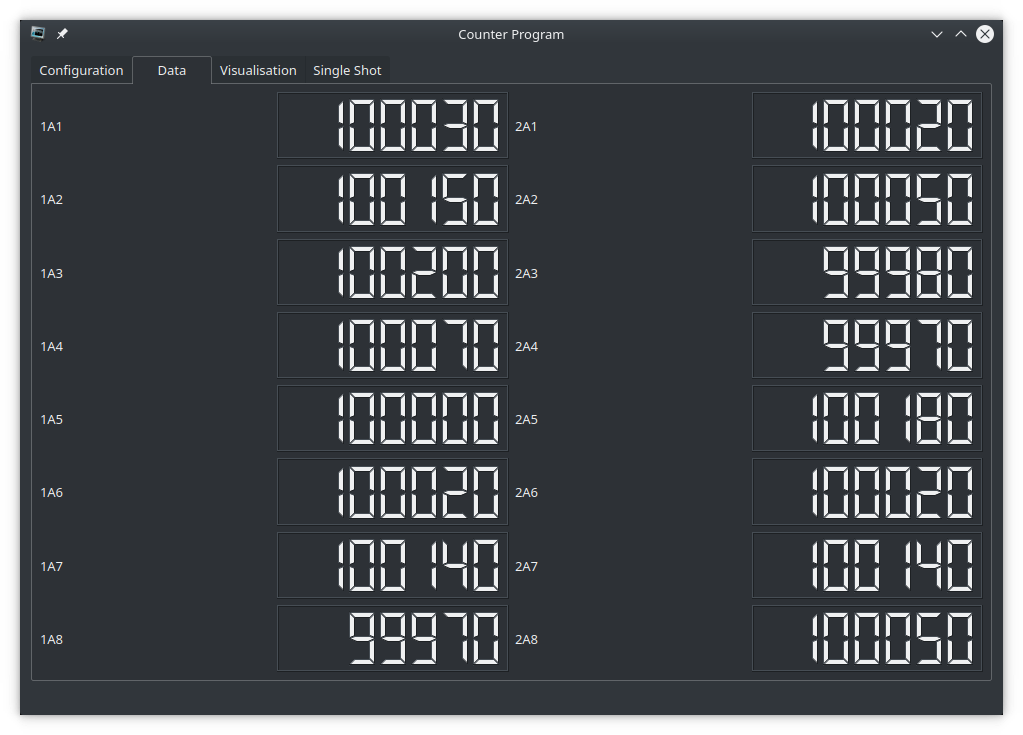
\includegraphics[width=0.49\textwidth]{GUI_digits.png}\par
        
        
        \end{multicols}\hfill
        
        \begin{multicols}{2}
        
        
        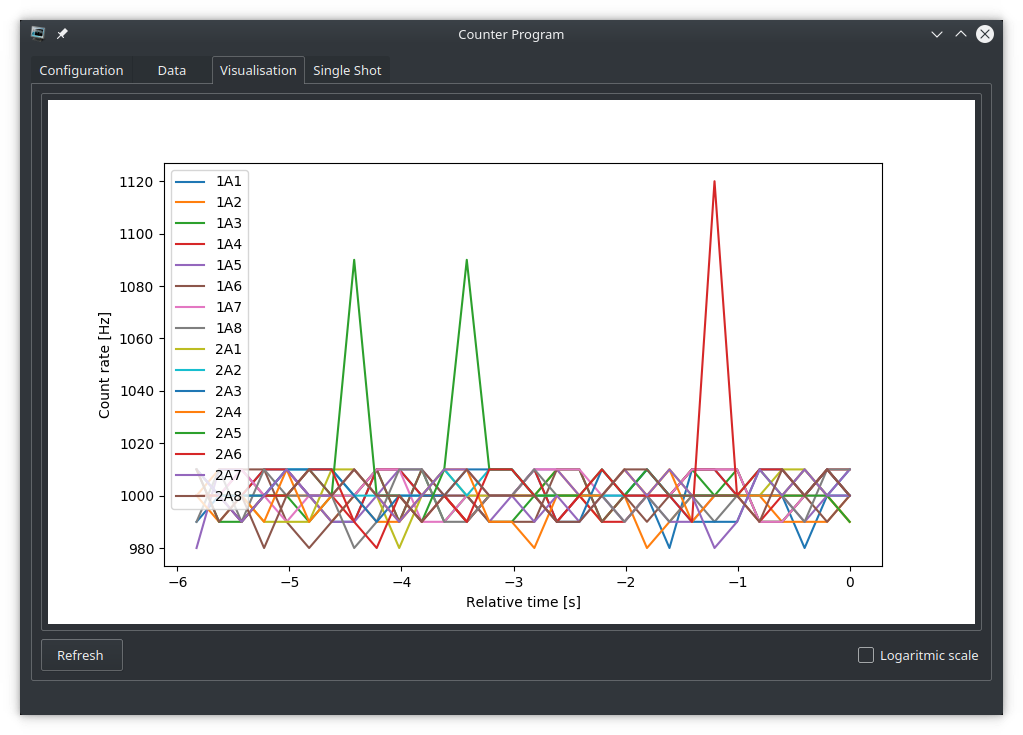
\includegraphics[width=0.49\textwidth]{GUI_VIS.png}\par
        
        
        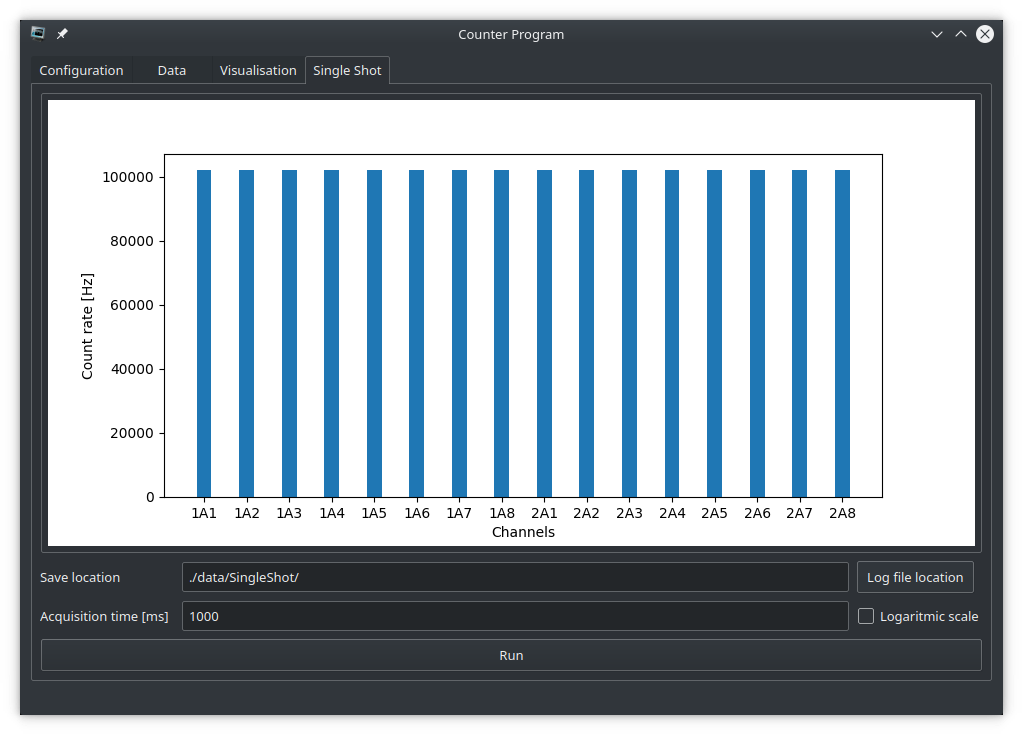
\includegraphics[width=0.49\textwidth]{GUI_SS.png}\par
        
        \end{multicols}
        \caption{Wygląd interfejsu użytkownika (linux)}
        \label{Gui pic}
        \end{figure}

Gotowy interfejs graficzny widoczny jest na rysunku \ref{Gui pic}. Jest on podzielony na cztery zakładki:
\begin{itemize}
        \item Configuration - miejsce pozwalające na rozpoczęcie pracy licznika, zatrzymanie i wszelką konfigurację dotyczącą pracy programu, 
        \item Data - prezentacja danych bieżących w postaci liczbowej, 
        \item Visualization - prezentacja danych w relatywnej dziedzinie czasu,
        \item Single Shot - zakładka odpowiedzialna za przeprowadzenie pojedynczego badania.
\end{itemize}

Za interfejs użytkownika odpowiedzialny jest główny wątek programu, instancje klasy QTimer\cite{doc pyqt} generują one sygnały aktualizujące dane licznika oraz sygnały aktualizacji wykresu zliczeń. 

Główny moduł zwany \textit{gui\_module} zapisuje informacje konfiguracyjne w instancji klasy \textit{ConfigurationData} która następnie jest wykorzystywana w komunikacji z mikrokontrolerem. Następujące parametry badania mogą być zmieniane:
\begin{itemize}
        \item Acquisision time (czas akwizycji) - przeliczany na ilość iteracji pętli czas akwizycji zliczeń. Czas ten podawany jest w milisekundach.
        \item Nr of averages (ilość uśrednień) - Jedną z funkcjonalności programu jest uśrednienie danych przed ich wizualizacją. Wartość tej liczby mówi jak dużo danych akwizycji zostanie użytych przed uśrednieniem wartości i wizualizacją. Liczba ta nie wpływa na dane zapisywane w plikach danych pomiarowych.
        \item Auto save period [mm:ss] (częstotliwość automatycznego zapisu) - czas podany w formacie [minuty:sekundy] po którym nastąpi automatyczne zapisanie danych. 
        \item Data location (ścieżka danych) - ścieżka pod którą będzie umieszczony folder z danymi. 
        \item Data save type (typ zapisu) - wybór zapisu danych w formacie JSON lub CSV.
        \item Arduino port (nazwa portu) - lista pozwalająca wybrać port szeregowy USB do którego podłączony został mikrokontroler. 
        \item Kontrola integratora 
        \begin{itemize}
                \item LOW Rate - ustalenie logicznej wartości lini LOW\_RATE układu RXHDR
                \item ENBLR - ustalenie logicznej wartości lini ENBLR układu RXHDR
        \end{itemize} 
\end{itemize}

Do generowania grafik zastosowana została biblioteka matplotlib\cite{doc matplotlib}. 

Przy wykresach znajduje się pole które po odznaczeniu pozwala na wizualizację danych w logarytmicznej sali częstotliwości zliczeń. Dodatkowo dodano funkcjonalność pozwalającą na odświeżenie wykresów i generację wizualizacji od nowa.

\paragraph*{}

Kod programu dostępny jest jako repozytorium GitHub pod adresem \url{https://github.com/SuroWka-Roch/WojSur_Masters_Deg}
